\documentclass[convert = false, tikz]{standalone}
\usepackage[utf8]{inputenc}
\usepackage{tikz}
\usetikzlibrary{automata, positioning, arrows}
 
\usepackage{../../../../style_automata}

% arara: pdflatex
% arara: latexmk: { clean: partial }
\begin{document}
\begin{tabular}{c}
    r=a: \\
    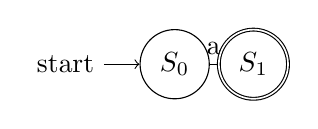
\begin{tikzpicture}
        \node[state, initial] (s0) {$S_0$};
        \node[state, accepting, right of=s0] (s1) {$S_1$};
        
        \draw (s0) edge[above] node{a} (s1);
    \end{tikzpicture}
    \end{tabular}
    \qquad % Adjust the horizontal space
    \begin{tabular}{c}
    r=\(\varepsilon\): \\
    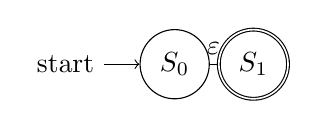
\begin{tikzpicture}
        \node[state, initial] (s0) {$S_0$};
        \node[state, accepting, right of=s0] (s1) {$S_1$};
    
        \draw (s0) edge[above] node{\(\varepsilon\)} (s1);
    \end{tikzpicture}
    \end{tabular}
\end{document}